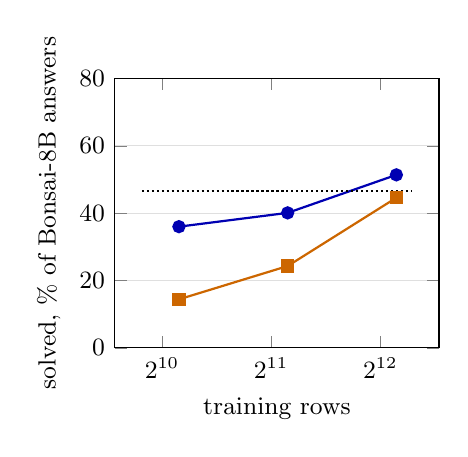
\begin{tikzpicture}
\begin{axis}[width=0.47\linewidth, height=5.0cm, xmode=log, log basis x=2, xlabel={training rows}, ylabel={solved, \% of Bonsai-8B answers},
  ymin=0, ymax=80, ymajorgrids, grid style={gray!25}, 
  tick label style={font=\small}, label style={font=\small}]
\addplot[blue!70!black, mark=*, thick] coordinates {(1139,36.0) (2271,40.1) (4528,51.4)};
\addplot[orange!80!black, mark=square*, thick] coordinates {(1139,14.4) (2271,24.3) (4528,44.6)};
\addplot[black, densely dotted, thick, domain=900:5000, samples=2] {46.6};
\end{axis}
\end{tikzpicture}
